\section{测试数据}

\subsection{实验简介}

实验部分采用了三个图数据集,其中有两个无向图和一个有向图,介绍如下:

\begin{enumerate}
    \item \textbf{aves-wildbird-network-3},带权无向图,来自AAAI论文开源数据\footnote{\url{http://networkrepository.com/aves-wildbird-network-3.php}}
    \item \textbf{Zachary karate club network} ,无权无向图,图领域的经典数据集\footnote{\url{http://konect.cc/networks/ucidata-zachary/}}
    \item \textbf{Intra-organisational networks},有向无权图,来自数据集网站\texttt{Tore Opsahl}\footnote{\url{https://toreopsahl.com/datasets/#Cross_Parker}}
\end{enumerate}

实验采用的评价指标是图内部权重与外部权重之商。
定义所有子图的内部连边之和为$I$,所有子图之间连边权重之和为$E$,则划分的质量为$I/E$。

\subsection{散列划分}

散列划分没有考虑到子图之间的连接关系,只是简单的根据哈希函数进行分区,因此效果较差。
下面的实验显示了分区数为$2$和$3$是的效果:

\begin{table}[htbp]
    \centering
    \begin{tabular}{cc}
    \hline
    分区数  & 划分性能 \\
    \hline
    2      & 0.9088310711082526 \\
    3      & 0.5066518381951788 \\
    \hline
    \end{tabular}
    \caption{散列划分在不同分区数量下的性能差异}
\end{table}

\subsection{Kernighan–Lin算法}

Kernighan–Lin算法在实验的初始阶段对数据集进行随机划分。
因为Kernighan–Lin算法对初始化数据集划分比较敏感,所以实验设置不同的随机种子的来初始化划分数据集。
在不同随机种子下,Kernighan–Lin算法的划分质量如下:

\begin{table}[htbp]
    \centering
    \begin{tabular}{cc}
        \hline
        seed  &划分性能\\
        \hline
        324   &9.353000586441842\\
        3241  &11.619001054402\\
        1234  &25.071660045156847\\
        \hline
    \end{tabular}
    \caption{不同的随机初始化对Kernighan–Lin算法性能的影响}
\end{table}

下图展示了不同随机初始化情况下Kernighan–Lin算法划分质量的变化。

\begin{figure}[htbp]
    \centering
    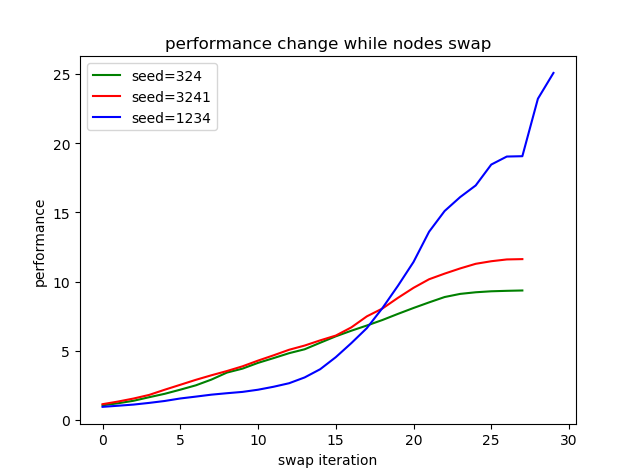
\includegraphics[width=0.55\linewidth]{figure/KL.png}
    \caption{不同随机初始化情况下Kernighan–Lin算法划分质量变化曲线}
    \label{}
\end{figure}
% \figure{../figure/KL.png}

由图可知,每次数据点的交换迭代都能带来性能的提高,所以Kernighan–Lin算法的贪心策略有效的。

\subsection{谱聚类}

谱聚类用幂迭代法计算归一化拉普拉斯矩阵的特征值和特征向量。
在进行幂迭代计算时,需要设置最大迭代次数。
现在用AAAI aves-wildbird-network-3数据集做测试。
下表展示了最大迭代次数为$2$、$10$、$20$三种情况下,谱聚类的图划分质量以及运行时间。

\begin{table}[htbp]
    \centering
    \begin{tabular}{ccc}
        \hline
        最大迭代次数 &划分性能&运行时间 \\
        \hline
        2           &39.32289045366845    &4.134 \\
        10          &70.58323798892366    &7.184 \\
        20           &70.58323798892366    &11.516 \\
        \hline
    \end{tabular}
    \caption{谱聚类性能、运行时间与最大迭代次数的关系(AAAI)}
\end{table}

通过观察上图,不难得出结论:在AAAI数据集上,谱聚类可以在$10$轮之内收敛。
过多地增加迭代次数对提高图划分的质量没有任何帮助,而适当降低迭代次数可以显著降低运行时间。

随后用Zachary数据集做进一步测试,使用不同的迭代次数。
实验结果如下图。

\begin{table}[htbp]
    \centering
    \begin{tabular}{ccc}
        \hline
    最大迭代次数 &划分performance      &运行时间 \\
        \hline
    20          &4.2                  &7.573 \\
    30          &5.5                   &9.28 \\
    40          &5.5                  &13.047 \\
        \hline
    \end{tabular}
    \caption{谱聚类性能、运行时间与最大迭代次数的关系(Zachary)}
\end{table}

由实验结果得,在Zachary数据集中需要$20$轮以上才会收敛。
综上所述,最大迭代次数需要在具体的数据集上先做一些试探性的实验才能确定。

\subsection{Metis算法}

\subsubsection{最大匹配策略实验}

这里对Metis算法粗化部分的匹配策略进行比较实验。
实际实验证明,使用原生的Heavy Edge匹配策略会导致数据点在多次粗化之后形成高度聚集,从而造成下一阶段中谱聚类的划分结果严重不平衡。
为了解决这个问题,本文提出可以用权重归一化来在一定程度上缓解这种不平衡划分。
下面固定参数$c=35$,分别测试了四种匹配策略下的图划分质量,包括
Heavy edge(HE)、Heavy Edge with Weight Normalization(HEWN)、Random Heavy Edge(RHE)、Random Heavy Edge with Weight Normalization(RHEWN)。

\begin{table}[htbp]
    \centering
    \begin{tabular}{cc}
        \hline
        策略        &划分性能\\
        \hline
        HE &53.95506559164985 \\
        HEWN &78.37563264477501 \\
        RHE &79.52152205384091 \\
        RHEWN &79.52152205384091 \\
        \hline
    \end{tabular}
    \caption{Metis中四种匹配策略下的划分性能(AAAI)}
\end{table}

从实验的结果,可以得出以下三个结论:
\begin{enumerate}
    \item 由于Heavy Edge划分不平衡,所以Metis算法的性能较差;
    \item 权重归一化技术(Weight Normalization)可以在一定程度上提高最终划分的性能;
    \item Random Heavy Edge算法的划分结果比较平衡,所以在使用权重归一化之后,其性能提高不明显;
\end{enumerate}

\subsubsection{参数$c$选取实验}

参数$c$控制粗化的程度。Metis算法的粗化阶段在节点数量小于等于$c*k$时停止。
一般来说参数$c$越大,图数据的粗化程度越低,信息损耗越少,划分的性能越高。
然而,参数$c$越大,对Metis划分阶段的算法性能要求就越高。
本系统瓶颈在粗化阶段,所以参数$c$越大,时间消耗越少。

\begin{table}[htbp]
    \centering
    \begin{tabular}{ccc}
        \hline
        c    &划分性能 &运行时间 \\
        \hline
        15 &77.94451753134379 &120.644 \\
        25 &79.37368802905935 &114.546 \\
        35 &79.52152205384091 &80.608 \\
        50 &79.52152205384091 &73.314 \\
        \hline
    \end{tabular}
    \caption{Metis算法的与运行时间与参数$c$的关系(AAAI)}
\end{table}

\subsubsection{谱聚类与Metis算法的横向对比}

下面分别比较当划分子图个数$k$为$2$个,$3$个的时候,谱聚类与Metis在三个数据集上面得到的图划分质量
在AAAI network上的谱聚类的最大迭代次数取$10$,Metis算法的$c$取$35$,
在Zachary network上谱聚类的最大迭代次数取$30$,Metis算法的$c$取$15$
在Intra-organisational networks上谱聚类最大迭代次数取$20$,Metis算法的$c$取$20$

\begin{table}[htbp]
    \centering
    \begin{tabular}{|c|c|c|c|c|}
        \hline
    &\multicolumn{2}{c|}{AAAI network} &\multicolumn{2}{c|}{Zachary network} \\
        \hline
    algorithm      &peformance           &运行时间   &peformance  &运行时间 \\
        \hline
    谱聚类          &70.58323798892366    &7.184      &5.5      &9.28\\
    Metis           &79.52152205384091    &80.608     &15.75    &16.455\\
        \hline
    \end{tabular}
    \caption{k=2时,三种数据集下谱聚类与metis的performance与运行时间的横向比较}
\end{table}


\begin{table}[htbp]
    \centering
    \begin{tabular}{ccc}
        \hline
        algorithm &peformance &运行时间\\
        \hline
        谱聚类   &4.0835509138381205  &7.402\\
        Metis   &4.607476635514018 &22.008\\
        \hline
    \end{tabular}
    \caption{Intra-organisational networks}
\end{table}

%%%%%%%%%%%%%%%%%%%%%%%%%%%%%%%%

\begin{table}[htbp]
    \centering
    \begin{tabular}{ccc}
        \hline
        algorithm                   &peformance           &运行时间\\
        \hline
        谱聚类             &25.157246974213972           &16.002   \\
        Metis             &34.0869985482627             &142.93\\
        \hline
    \end{tabular}
    \caption{k=3时,AAAI数据集下谱聚类与metis的performance与运行时间的横向比较}
\end{table}

可以看出,在划分子图个数为$2$个和$3$个的时候,Metis在不同数据集上,划分的性能都要比谱聚类好,但是Metis的运行时间要显著高于谱聚类算法。
